% !TEX encoding = UTF-8 Unicode

\documentclass[11pt]{beamer}

\usepackage{color}
\usepackage{url}
\usepackage{amsthm}
\usepackage[T2A]{fontenc} % enable Cyrillic fonts
\usepackage[utf8]{inputenc} % make weird characters work
\usepackage{graphicx}
\usepackage{subcaption}
\usepackage{amsmath}
\usepackage{comment}
% \graphicspath{ {.} }

\usepackage[english,serbian]{babel}
%\usepackage[english,serbianc]{babel} %ukljuciti babel sa ovim opcijama, umesto gornjim, ukoliko se koristi cirilica

%\usepackage[unicode]{hyperref}
%\hypersetup{colorlinks,citecolor=green,filecolor=green,linkcolor=blue,urlcolor=blue}

\newtheorem*{tvrdjenje}{Tvrđenje}
\newtheorem*{hipoteza}{Hipoteza}
\theoremstyle{definition}
%\newtheorem{primer}{Пример}[section] %ćirilični primer
\newtheorem{primer}{Primer}[section]

\mode<presentation>{\usetheme{Warsaw}}
%\usecolortheme{lily}
\usefonttheme{serif}

%\AtBeginSection[]{
%\begin{frame}
%\frametitle{Sadržaj}
%\tableofcontents[currentsection]
%\end{frame}
%}

%\renewcommand{\abstractname}{Apstrakt} %pisace Sazetak ako se ne ukljuci ova naredba

\title{Primena mašinskog učenja u verifikaciji softvera}

\author[\hspace{-0.8em}N. Dimitrijević, R. Đorđević, L. Živanović, D. Špadijer]
		{Nikola Dimitrijević\\ % \footnote{nikoladim95@gmail.com}\\
        Rastko Đorđević\\ % \footnote{mi14078@alas.matf.bg.ac.rs}\\
        Luka Živanović\\ % \footnote{mi14164@alas.matf.bg.ac.rs}\\
        Dimitrije Špadijer} % \footnote{mm11021@alas.matf.bg.ac.rs}\\}
\date{14. maj 2018.}

\begin{document}
\begin{frame}
\titlepage
\end{frame}

\section{Uvod}
\label{sec:uvod}
\begin{frame}
\frametitle{Uvod}
\begin{itemize}
\item Softverska rešenja su prisutna svuda
\item Veoma je važno da taj softver bude ispravan
\item Verifikacija softvera se bavi proverom ispravnosti softvera
\item Mnoga ograničenja u verifikaciji koja se teško prevazilaze
\item Mašinsko učenje je popularno i s puno uspeha
\item Primene mašinskog učenja u verifikaciji
\end{itemize}

\end{frame}
\section{Verifikacija softvera}
\label{sec:verifikacija}
\begin{frame}
\frametitle{Verifikacija softvera}
\begin{itemize}
\item Oblast razvoja softvera koja se bavi proverom ispravnosti softvera
\item Potpuno ispravan i delimično ispravan softver
\item Razlika je u tome da li se zaustavlja za svaki ulaz
\item Zbog neodlučivosti halting problema, uglavnom se proverava delimična ispravnost
\item Dinamička i statička verifikacija \cite{milena}
\end{itemize}
\end{frame}

\subsection{Dinamička verifikacija softvera}
\label{subsec:dinamicka}
\begin{frame}
\frametitle{Dinamička verifikacija softvera}
\begin{itemize}
\item Provera ispravnosti softvera tokom njegovog izvršavanja
\item Testiranje $\subset$ dinamička verifikacija
\item Testiranjem se dokazuje prisustvo, ali ne i odsustvo grešaka
\item Dobar skup testova obezbeđuje sigurnost i poverenje u softver
\item Debagovanje --- drugi najčešći vid dinamičke verifikacije
\end{itemize}
\end{frame}

\subsection{Statička verifikacija softvera}
\label{subsec:staticka}

\begin{frame}
\frametitle{Statička verifikacija softvera}
\begin{itemize}
\item Provera ispravnosti softvera bez njegovog pokretanja
\item Pregled koda i automatska verifikacija
\item Uvid u kvalitet koda i u propuste
\item Tehnike:
	\begin{itemize}
		\item \textbf{Analiza toka podataka} (eng. \textcolor{red}{data flow analysis})
		\item \textbf{Apstraktna interpretacija} (eng. \textcolor{red}{abstract interpretation})
		\item \textbf{Simbolička analiza} (eng. \textcolor{red}{symbolic analysis})
		\item \textbf{Proveravanje ograničenih modela} (eng. \textcolor{red}{Bounded model checking}), koja se najviše koristi za verifikaciju logičkih kola.
	\end{itemize}
\end{itemize}
\end{frame}

\section{Mašinsko učenje}

\begin{frame}
\frametitle{Mašinsko učenje}

\begin{block}{Definicija}
\textcolor{red}{Mašinsko učenje} bavi se proučavanjem indukcije, odnosno generalizacije, čime formalizuje uopštavanje od uzorka određene veličine ka univerzalnim zaključcima \cite{bishopML}.
\end{block}

\begin{itemize}
\item Mašinsko učenje postiže rezultate superiorne u odnosu na rezultate ljudskih eksperata
\item Pogodno za probleme koji se teško definišu, a izuzetno lako rešavaju, i u kojima je prihvatljiva poneka greška
\item Kako se primenjuje na verifikaciju, ako se dopuštaju greške?
\end{itemize}

\end{frame}

\begin{frame}
\frametitle{Mašinsko učenje}
\begin{itemize}
\item Tri oblasti mašinskog učenja:
	\begin{itemize}
	\item \textbf{Nadgledano učenje} (eng. \textcolor{red}{supervised learning})
	\item \textbf{Nenadgledano učenje} (eng. \textcolor{red}{unsupervised learning})
	\item \textbf{Učenje uslovljavanjem} (eng. \textcolor{red}{reinforcement learning})
	\end{itemize}
\item Nadgledano učenje: za svaki ulaz postoji i željeni izlaz
\item Nenadgledano učenje: algoritmu se ostavlja da sam otkrije strukturu u podacima
\item Učenje uslovljavanjem: oblast između prethodne dve
\end{itemize}
\end{frame}

\begin{frame}
\frametitle{Koraci}
\begin{itemize}
\item Analiza problema i podataka nad kojim će tehnike biti primenjene
\item Izbor odgovarajućih modela
\item Pretprocesiranje podataka i treniranje modela nad tako obrađenim podacima
\item Evaulacija istreniranog modela i mera njegove korisnosti
\end{itemize}
\end{frame}

\subsection{Evaluacija modela i mere kvaliteta}
\begin{frame}
\frametitle{Evaluacija modela i mere kvaliteta}
\begin{itemize}
\item Numeričko predstavljanje sposobnosti predviđanja datog modela na određenoj skali
\item Direktno se oslanja na mere kvaliteta: \textcolor{red}{tačnost}, \textcolor{red}{preciznost}, \textcolor{red}{odziv} i \textcolor{red}{F1 mera}
\item Mere su izvedene iz matrice konfuzije
\end{itemize}

\begin{table}[h]
	\centering
	\begin{tabular}{ |c|cc| }
		\hline
		Stvarno $\backslash$  Predviđeno & Pozitivno & Negativno \\
		\hline
		Pozitivno & Stvarno Pozitivno & Lažno Negativno \\
		Negativno & Lažno Pozitivno & Stvarno Negativno \\
		\hline
	\end{tabular}
	\caption{Matrica konfuzije}
	\label{table:matrica_konfuzije}
	%\caption{ tabelica stagod}
\end{table}

\end{frame}

\begin{frame}
\frametitle{Evaluacija modela i mere kvaliteta}
\begin{itemize}
\item Tačnost: udeo uspešno klasifikovanih instanci u odnosu na ukupan broj instanci
\item Preciznost: udeo ispravno pronađenih pozitivnih instanci u svim instancama koje su proglašene za pozitivne
\item Odziv: udeo ispravno pronađenih pozitivnih instanci u svim zaista pozitivnim instancama
\item F1 mera: harmonijska sredina preciznosti i odziva
\end{itemize}
\end{frame}

\section{Odabrani problemi statičke verifikacije}
\label{sec:naslovN}

\subsection{Formalna verifikacija softvera}
\label{subsec:formalna-verifikacija}
\begin{frame}
\frametitle{Formalna verifikacija}
\begin{itemize}
\item Formalni, matematički pristup verifikaciji \cite{verify}
\item $P$ program, $T$ skup testova, $S$ specifikacija
$$(\forall t\in T)\ [prolazi(P,t)\wedge S\models t]\Rightarrow P\equiv S$$
\item Dva česta problema:
	\begin{itemize}
	\item Pronaći \textcolor{red}{adekvatan} skup testova $T$
	\item Proveriti tačnost konjukcije $prolazi(P,t)\wedge S\models t$ (\textcolor{red}{problem proročišta})
	\end{itemize}
\item Prevazilaze se primenom mašinskog učenja i indukovanje teorije koja odgovara datim podacima
\item Matematički pojmovi iz teorije jednačina (eng. \textcolor{red}{equational theory} \cite{equationaltheory})
\end{itemize}
\end{frame}

\begin{frame}
\frametitle{Formalna verifikacija}
\begin{itemize}
\item Centralni pojam je $\Sigma$-teorija; program posmatramo kao $\Sigma$-teoriju
\item \textcolor{red}{Koherentan} i \textcolor{red}{adekvatan} skup testova
\item Na osnovu skupa testova indukuje se teorija $H$
\end{itemize}

\begin{block}{Tvrđenje}
Ako je $S$ specifikacija, $P$ program i $T$ adekvatan i koherentan skup testova, onda je $P$ ispravan u odnosu na specifikaciju $S$.
\end{block}

\begin{itemize}
\item Primeri sa stekom; adekvatan i neadekvatan skup testova
\end{itemize}
\end{frame}


% Rastkov rad
\subsection{Formalna verifikacija softvera}
\label{subsec:formalna-verifikacija}
\begin{frame}
\frametitle{Rastkov rad}
blablabla
\end{frame}

% Nikolin rad
\subsection{Formalna verifikacija softvera}
\label{subsec:formalna-verifikacija}
\begin{frame}
\frametitle{Nikolin rad}
Pravljenje modela mašinskog učenja za detekciju grešaka korišćenjem izvornih kodova.

1. Kako transformisati izvorni kod u odgovarajući format za klasifikatore?
2. Kako trenirati te klasifikatore i koje podatke treba koristiti?
3. Koje su karakteristike potrebne algoritmu i koji je najbolji za dati problem?

Od javno dostupnih repozitorijuma se može lako dobiti veliki skup za treniranje upoređivanjem verzija datoteka.

Koristi se program CMore koji izdvaja stanja programa analizirajući izvorni kod
i kao izlaz daje odgovarajucu ARFF datoteku.

Potom program Holmes od ARFF datoteke ispravnog koda i onog sa greškom pravi novu ARFF datoteku
gde su samo razlike zadržane.
\end{frame}

% Nikolin rad
\subsection{Formalna verifikacija softvera}
\label{subsec:formalna-verifikacija}
\begin{frame}
\frametitle{Nikolin rad}
WEKA - biblioteka mašinskog učenja.
Moze iskoristiti jednu ARFF datoteku kao ulaz za vise razlicitih algoritama.

Analiza pogodnosti daje rezultate poredjenja 71 klasifikatora.

Među najboljim su
Neuronska mreža MultiLayerPerceptron
Najbliži susedi Ibk
Stabla ADABoost
\end{frame}



% Lukin rad
\subsection{Formalna verifikacija softvera}
\label{subsec:formalna-verifikacija}
\begin{frame}
\frametitle{Lukin rad}
blablabla
\end{frame}


\subsection{Učenje statičkog analizatora iz podataka}
\label{subsec:staticki-analizator}

\subsection{Od izvornog koda do istreniranih modela}
\label{subsec:pregled}

\section{Primena mašinskog učenja u dinamičkoj verifikaciji}
\label{sec:dinamcikaPrimena}

\subsection{Onlajn testiranje korišćenjem učenja uslovljavanjem }

\section{Zaključak}
\label{sec:zakljucak}






























\begin{comment}

% ==============================================================================
\subsection{Učenje statičkog analizatora iz podataka}
\label{subsec:staticki-analizator}
% ==============================================================================

% šta su statički analizatori
Da bi bili korisni u praksi, moderni statički analizatori moraju precizno
modelovati ne samo efekte naredbi programskog jezika, već i efekte biblioteka
i okvira (eng. \emph{frameworks}) koji mogu da se koriste. Ručno adresiranje ovih izazova
je izuzetno teško zbog priliva novih biblioteka, kao i kompleksnosti i
netrivijalnosti sveobuhvatne analize. U ovoj sekciji biće opisan nov
automatski pristup za kreiranje statičkih analizatora koji se oslanja na
korišćenje tehnika mašinskog učenja. Detaljan prikaz pristupa se može naći
u radu \cite{staticAnalyzer}.

% formalan prikaz problema
Formalan prikaz problema koji će biti obrađen u nastavku glasi: za dati
specifični domenski jezik $\mathcal{L}$, koji služi za opis pravila analize,
skup $\mathcal{D}$ programa u nekom programskom jeziku (npr. JavaScript), i
funkciju apstrakcije $\alpha$ koja definiše kako se konkretna ponašanja
apstrahuju, cilj je naučiti analizator $pa$ koji pripada skupu $\mathcal{L}$
takav da se programi iz $\mathcal{D}$ analiziraju maksimalno precizno u odnosu
na $\alpha$.


% prvi problem
Postoje dva ključna izazova pri izgradnji statičkog analizatora. Prvo, statički
analizatori su tipično opisani pomoću pravila, dok postojeće te\-hni\-ke mašinskog
učenja kao rezultat daju kombinaciju postojećih pravila. Ako bi se ove tehnike
primenile na programsku analizu \cite{predictingProgramProperties} dobijena
pravila ne bi bila interesantna. Iz tog razloga uvodi se specifični domenski
jezik za opis pravila analize, nad kojim se mogu učiti nova pravila analize.


% detaljan opis rešenja prvog problema
Izuzetno važan problem prilikom učenja programskih analizatora je ogromna količina
programa nad $\mathcal{L}$ zato što je broj kombinacija grana i potprograma previše veliki.
Međutim, može se primetiti da se elementi skupa L mogu predstaviti kao drvo, čiji
unutrašnji čvorovi predstavljaju čuvare, koji su kondicionalne naredbe, a čiji
listovi predstavljaju akcije koje se mogu izvršiti. Koristeći ovo zapažanje problem
učenja analizatora u L se može predstaviti kao problem učenja stabla odlučivanja,
što omogućava korišćenje postojećih algoritama mašinskog učenja za
rešenje datog problema.

Prema tome, ID3 \cite{id3} algoritam se proširuje kako bi mogao da obradi akcije
programa u listovima, i da obezbedi korektnost rezultujuće analize $pa$ nad
$\mathcal{L}$. Kao i ID3, njegova modifikacija je pohlepna procedura koja gradi
stablo odlučivanja odozgo-nadole, pritom lokalno maksimizujući metriku koja se
naziva informaciona dobit. Za dati predikat $g$, koji odgovara čuvaru,
informaciona dobit kvantifikuje koliko se popravlja procena svih programa u
skupu $\mathcal{D}$, ukoliko se analiza proširi deljenjem skupa podataka
pomoću predikata $g$.


% drugi problem
Drugi znatno izazovniji problem pri izgradnji statičkog analizatora je
kako izbeći učenje statičkog analizatora koji se ponaša dobro
na podacima za treniranje $\mathcal{D}$, ali koji ne uspeva da se
generalizuje na nove programe van skupa $\mathcal{D}$. Ovaj problem se u mašinskom
učenju naziva preprilagođavanje. Standardne tehnike koje se koriste za suočavanje
sa ovim problemom \cite{statisticalLearningTheory}, kao što je regularizacija su
nedovoljne u ovom slučaju. Osnovna ideja regularizacije je da pojednostavi skup
modela koji se mogu naučiti, što je u kontradikciji sa neophodnom osobinom
statičkog analizatora da ispravno kategoriše granične slučajeve. Ovaj problem
se rešava procedurom učenja vođenog kontraprimerima koja generiše nove
programe, koristeći programsku semantiku, za koje naučeni analizator daje
pogrešne rezultate i koji služe za dalje učenje.


% detaljan opis rešenja drugog problema
Ključna komponenta ovog pristupa je proročište (eng. \emph{oracle}) koje brzo može
testirati korektnost statičkog analizatora, i ako je analizator korektan
pronaći kontraprimere. Proročište kao ulaz uzima analizator $pa$ i skup
podataka $\mathcal{D}$ koji je korišćen prilikom učenja analizatora $pa$
i kao izlaz vraća kontraprimere programa na kojima se analizator ne
ponaša korektno.

Najveći problem koji se mora rešiti je brz pronalazak kontraprimera u prostoru
pretrage svih mogućih programa. Kao što je pokazano u radu \cite{staticAnalyzer}
nasumično generisanje kontraprimera ne funkcioniše usled prirode prostora
pretrage koji može biti čak i beskonačan. Pretraga se ubrzava dizajnom
proročišta opšte namene koje je bazirano na idejama modernih tehnika testiranja
\cite{testing}.

Novi programi se generišu izvođenjem modifikacija nad programima u skupu
$\mathcal{D}$. Ove modifikacije se pažljivo biraju eksploatisanjem strukture
trenutne analize $pa$ na dva načina: (i) da bi se izabrao određeni program i
pozicija za modifikaciju, i (ii) da bi se odredila modifikacija koja će se
izvršiti na toj poziciji.


% primene
Metoda je pokazana kroz implementaciju pristupa i evaluaciju na problemu analize
pravila jezika JavaScript. Naučena pravila za pokazuje-na analizu, kao i za
analizu alokacionih mesta, su izuzetno interesantna. Neka od naučenih pravila su propuštena od
strane postojećih najmodernijih ručno podešenih statičkih analizatora kao što
su Flow \cite{flow} koji koristi Facebook, i TAJS \cite{tajs}.

% doprinosi rada
Glavni doprinosi opisanog rada su sledeći. Metod učenja pravila sta\-ti\-čkih
analizatora koji dobro generalizuje zbog pažljivog generisanja kontraprimera
nad pravilima koja su naučena u tom trenutku. Algoritam mašinskog učenja baziran
na drvetu odluke za učenje pravila analize iz podataka, koji uči da
pre-aproksimira kada skup podataka ne može da se obradi precizno.

\subsection{Od izvornog koda do istreniranih modela}
\label{subsec:pregled}

Rad \cite{staticFeatures} predlaže rešenje za generisanje ulaznih podataka za algoritme mašinskog učenja na osnovu
izvornog koda kako bi se napravio inteligentni metod detekcije grešaka.

Bitno je prvo definisati kakvim tipovima grešaka se posvećuje pažnja u okviru metoda.
Iako postoje drukčije greške selekcija je vršena prema važnosti, odnosno prema tome
koliku štetu mogu da uzrokuju i mogućnost da budu detektovane računarskim alatom. Izabrani tipovi grešaka su:
% može se navesti iz koje knjige su uzete !!!!
%\begin{itemize}
prekoračenje bafera,
upravljanje memorijom,
dereferenciranje null pokazivača,
kontrola toka i
konverzija označene celobrojne vrednosti u neoznačenu.
%\end{itemize}

Korišćen je WEKA softver koji je kolekcija algoritama mašinskog u\-če\-nja.
U bogat skup funkcionalnosti koje pruža WEKA spada:
%lista
%\begin{itemize}
pretprocesiranje podataka i vizuelizacija,
selekcija atributa,
algoritmi klasifikacije,
algoritmi predviđanja,
algoritmi klasterovanja,
pravila asocijacije i
tehnike evaluacije.
%\end{itemize}


Za dati problem su najbitniji selekcija atributa i razni algoritmi klasifikacije i predviđanja.
Prvi prikazuju koji od brojnih elemenata ulaznog vektora su zapravo uključeni u proces donošenja odluke a koji nisu, dok
drugi klasifikuju odnosno predviđaju ispravnost na osnovu ulaza.
Međutim, najbitnija prednost koju pruža WEKA u odnosu na ostale dostupne alate je mogućnost da se koristi
jedan standardizovani format ulaza za sve raspoložive algoritme učenja što omogućava da se koristi jedan ulaz kako bi se isprobale
razne mogućnosti.

Ulaz koji koristi WEKA je u formatu ARFF.
ARFF datoteke se sastoje od nabrajanja atributa odnosno njihovih imena i tipova, a potom navođenja svih instanci koje se prosleđuju algoritmima.

Glavni problem koji se rešava se može podeliti u tri potproblema koji su:
%list
\begin{enumerate}
\item Kako transformisati izvorni kod u odgovarajući format za klasifikatore?
\item Kako trenirati te klasifikatore i koje podatke treba koristiti?
\item Koje su karakteristike potrebne algoritmu i koji je najbolji za dati problem?
\end{enumerate}



Odgovor na prvo pitanje je softver ``CMore'' \cite{staticFeatures}, program koji može da pretvori izvorni kod programskog
jezika C u ARFF datoteku. Glavna ideja je da treba da bude u mogućnosti da prati tok izvršavanja programa
i uhvati stanja svih uključenih promenljivih. Pošto su zapamćena sva stanja moguće je otkriti više vrsta
grešaka pristupa memoriji.

Prvi deo izvršavanja je učitavanje datoteke u memoriju i njena obrada kako bi se izvukli
razni elementi i ubacili u skladište nazvano ``Mozak''.
Mozak sadrži listu svih poznatih tipova, struktura, konstanti i globalnih promenljivih unutar analizirane datoteke,
ali najbitnije je što pamti sve funkcije i njihove parametre.

U drugom delu se prati tok izvršavanja i određuje
priroda svake naredbe, što bi moglo biti dodela, deklaracija, poziv funkcije ili nešto drugo.
Sve vreme mora da se motri na sve sakupljene informacije i da se po potrebi dopisuju instance na kraj ARFF fajla
(koji je ulaz za algoritme mašinskog učenja).


Za treniranje je potreban veliki broj različitih izvornih kodova, a pritom je potrebno obeležiti greške i imati verzije koda kod kojih je uklonjena greška.
Izvorni kodovi od kojih se prave ulazi za treniranje su pokupljeni sa javno dostupnih repozitorijuma.
Na taj način se skupi velika količina datoteka, a pritom je moguće dobiti primere sa greškom i bez greške tako što se posmatraju različite verzije datoteka.

Na prvi pogled je dovoljno uzeti izlaz programa CMore u ARFF formatu za datoteku sa greškom i bez nje.
Međutim, CMore nema uvid u to šta je greška nego analizira celu datoteku.
Zbog toga generiše izlaze koji mogu imati više hiljada linija od kojih je većina nastala od ispravnih delova koda.
Potrebno je izdvojiti samo one linije koda koje su dovele do greške i njihove parove bez te greške.
Za tu svrhu se koristi program ``Holmes'' \cite{staticFeatures} koji upoređuje dve ARFF datoteke i na izlazu se dobiju dve nove ARFF datoteke koje sadrže samo potrebne  instance.

Nakon što se svi modeli mašinskog učenja istreniraju vrši se analiza pogodnosti
koja vraća listu pogodnih modela tako što analizira njihovu preciznost, stopu lažno pozitivnih i lažno negativnih.
U nastavku su prikazani rezultati poređenja 71 klasifikatora, a na slikama su prikazani samo oni koji su se najbolje pokazali. Cela procedura je urađena dva puta, s tim što je drugi put umanjen broj atributa uključenih u proces.

Među 7 najboljih klasifikatora sa slike \ref{fig:acc} se nalaze tri zasnovana na najbližim susedima (``Ib1'', ``Ibk'', ``NNge''), tri zasnovana na stablima
(``LMT'', ``RotationForest'' i ``ADABoost'' primenjen na ``BFTree'') i jedan zasnovan na neuronskim mrežama (``MultiLayerPerceptron'').
Na slici  \ref{fig:falsePos} se vidi isti trend kao i na slici  \ref{fig:acc}: smanjenjem broja atributa algoritmi zasnovani na stablima se lošije ponašaju dok algoritmi najbližih suseda i ``MultiLayerPerceptron'' daju bolje rezultate.



Prema rezultatima dobijenim u  \cite{baca} vrlo je bitno da alat statičke analize ima malo lažno pozitivnih.
U slučaju mnogo pogrešnih uzbuna programeri počinju da ignorišu te signale, ili još gore: kako bi izbegli upozorenja alata menjaju ispravan kod što dovodi do potencijalno
 novih grešaka. Na slici \ref{fig:falseNeg} se vidi da je ``NNge'' najbolji, što je i očekivano s obzirom na prilično
loše performanse što se tiče lažno pozitivnih.



% ==============================================================================
\section{Primena mašinskog učenja u dinamičkoj verifikaciji}
\label{sec:dinamcikaPrimena}
% ==============================================================================

Priroda algoritama mašinskog učenja mnogo više odgovara problemima koji se sreću
u dinamičkoj verifikaciji softvera. Stoga može se naći pregršt primena mašinskog
učenja u ovoj oblasti. Radi potpunosti, u nastavku će biti opisana jedna od tih
primena, koja se oslanja na učenje uslovljavanjem.


% ==============================================================================
\subsection{Onlajn testiranje korišćenjem učenja uslovljavanjem }
% ==============================================================================

Programi koji su reaktivni, naročito ako su distribuirani, mogu se ponašati nedeterministički. Neki faktori, poput redosleda završavanja niti nisu pod potpunom kontrolom testera, ali se njihovo ponašanje može modelovati stablom odlučivanja. Ipak, veličina tog stabla može da postane izuzetno velika za pretragu, pa se pribegava tehnikama onlajn testiranja.

Onlajn testiranje je tehnika u kojoj se kreiranje testa i njegovo izvršavanje rade u istom algoritmu. Može biti pogodnije od oflajn testiranja za reaktivne sisteme zato što se može dinamički prilagoditi za vreme izvršavanja tako da pokrije najrelevantnija ponašanja, umesto svih mogućih, što je obično nemoguće. Onlajn testiranje spada u skup testiranja baziranih na modelu (eng. \emph{model-based testing}), gde tester koristi model da detektuje razlike između impelementacije pod testom (eng. \emph{implementation under test - IUT}) i modela.

Razlikovaćemo poteze testera od IUTa. Akcije testera ćemo nazivati kontrolisane akcije, dok ćemo akcije IUTa nazivati posmatrane akcije. Greška usklađenosti nastaje kada IUT odbije kontrolisanu akciju modela ili kada model odbije posmatranu akciju IUTa.

Stanja modela čine memorijske lokacije programa koje su preslikane u konačni skup vrednosti.
Pravila ažuriranja su konačan skup funkcija koje preslikavaju vrednosti iz domena stanja u domen stanja. Pravilo ažuriranja $p$ može biti parametrizovano parametrima $\bar{x}$.
Instanciranje p[$\bar{x}$] ulaznim vrednostima $\bar{v}$ odgovarajućeg tipa, obeležava se p[$\bar{v}$].
Generalno, pravila ažuriranja mogu biti nedeterministička, tako da za isto ulazno stanje i vrednosti, može da ima različita izlazna stanja. Da bismo to modelovali, definišemo relaciju $[[p]] \subseteq Stanja \times Vrednost^n \times Stanja$.
Kada je p determinističko, [[p]] smatramo funkcijom [[p]]: $Stanja \times Vrednost^n  \rightarrow Stanja$

Čuvar $\varphi$ je formula koja zavisi od stanja. Može sadržati slobodne logičke promenljive $\bar{x} = x_1, x_2,..., x_n$ i takvo označavamo sa $\varphi(\bar{x})$. $\varphi$ je zatvoreno ako nema slobodnih varijabli. Zatvorena formula $\varphi$ ima istinitosnu interpretaciju u stanju $s \models \varphi$. Čuvano pravilo ažuriranja je par $(\varphi, p)$ i ono limitira primenu p na stanja i argumente koji zadovoljavaju $\varphi(\bar{v})$.

Model programa P sadrži sledeće komponente:
%\begin{itemize}
prostor stanja $Stanja$,
prostor vrednosti $Vrednosti$,
inicijalno stanje $s_0 \in Stanja$,
konačni skup simbola akcija $\Sigma$ podeljen u dva disjunktna podskupa ($\Sigma_c$ kontrolisanih akcija i $\Sigma_o$ posmatranih akcija),
familija $(\varphi_f, p_f) f \in \Sigma$ čuvanih pravila ažuriranja,
arnost funkcije f je broj ulaznih parametara $p_f$ i
arnost reset pravila je 0 i $[[p_{Reset}]](s) = s_0$ za sve $s \models \varphi_{Reset}$.
%\end{itemize}
P je determinističko, ako za svako $f \in \sigma, p_f$ je determinističko. \\

Akcija $f$ ima oblik $f(v_1,...,v_n)$, gde je $f$ $n$-arni akcijski simbol a svako $v_i$ vrednost koja odgovara ulaznom parametru $p_f$. Kažemo da je akcija $f(\bar{v})$ dozvoljena u stanju $s$ ako $s \models \varphi(\bar{v})$. Primetimo dva specijalna slučaja: kada je reset uvek zabranjen $(\varphi_{Reset} = false)$, kada je definicija $p_{Reset}$ irelevantna, i slučaj kada je reset uvek dozvoljen $(\varphi_{Reset} = false)$, i tada $p_{Reset}$ mora da bude definisana tako da iz svakog stanja može da uspostavi početno stanje.

I IUT i model posmatramo kao interfejs automate (eng. \emph{interface automata}) kako bismo formalno uspostavili vezu između njih \cite{interfaceAutomata}.
Interfejs automat M ima sledeće komponente:
\begin{itemize}
\item Skup stanja $S$
\item Neprazan podskup početnih stanja $S_{init}$ skupa $S$
\item Disjunktni skupovi kontrolisanih akcija $A_c$ i posmatranih akcija $A_o$
\item Dozvoljavajuće funkcije $\Gamma_c$ i $\Gamma_o$ podskupova $A_c$ i $A_o$, redom.
\item Prelazna funkcija $\sigma$ koja slika ulazno stanje i dozvoljavajuću akciju u izlazno stanje
\end{itemize}

Neka je P deterministički model $(Stanja, Vrednosti, s_0, \Sigma, \Sigma_c, \Sigma_0, Reset,\\ (\varphi_f, p_f)f \in \Sigma)$. Prema prethodnoj definiciji, intefejs automat P izgleda:

\begin{itemize}
\item $S_{[[P]]} = States$
\item $S^{init}_{[[P]]} = \{s_0\}$
\item $A^c_{[[P]]} = \{ f(\bar{v}) | f \in \Sigma^c, \bar{v} \subseteq Values \}$
\item $A^o_{[[P]]} = \{ f(\bar{v}) | f \in \Sigma^o, \bar{v} \subseteq Values \}$
\item $\Gamma^c_{[[P]]} = \{ f(\bar{v}) \in A^c_{[[P]]} | s \models \varphi_f(\bar{v}) \}$
\item $\Gamma^o_{[[P]]} = \{ f(\bar{v}) \in A^o_{[[P]]} | s \models \varphi_f(\bar{v}) \}$
\item $\sigma_{[[P]]}(s, f(\bar{v})) = [[P_f]](s, \bar{v}) (for f \in \Sigma, s \in States, s \models \varphi_f(\bar{v}))$
\end{itemize}

\noindent
Algoritam:

IUT i model, su oba predstavljeni kao interfejs automati.
Kako smo formalno definisali strukture modela, ostaje još da opišemo način izbora naredne akcije u algoritmu:
\begin{itemize}
\item Ukoliko nema mogućih akcija\\ prekini trenutni test.
\item Ukoliko nema mogućeg izbora za kontrolisanu akciju\\ vrati posmatranu.
\item Ukoliko nema mogućeg izbora za posmatranu akciju\\ vrati kontrolisanu.
\item Inače\\ izaberi između kontrolisane i posmatrane akcije.
\end{itemize}

Algoritam prati težine transakcija u trenutnom testu. Sledeća kontrolisana akcija se bira iz nepraznog skupa dozvoljenih akcija koristeći datu strategiju:

Za ovaj problem koristićemo algoritam mašinskog učenja koji spada u učenje uslovljavanjem, o kome su osnove date ranije u radu.
Cena testa se povećava srazmerno broju koraka kako bi se pokrio zadati procenat svih ponašanja. Iscrpno pokrivanje svih ponašanja je najčešće nemoguće. Umesto da posmatramo minimizaciju cene, možemo pretpostaviti da imamo fiksne resurse i da maksimizujemo procenat pokrivenih ponašanja. Bitno je da minimizujemo broj vraćanja u početno stanje (eng. \emph{backtracking}), zato što to može biti skupa operacija. %ONLINE

Odabir sledeće akcije:
\begin{itemize}
\item Najjeftinija: \\
Biramo akciju koja najmanje košta, odnosno ima najveću nagradu.

\item Nasumična: \\
Biramo akciju na nasumičan način

\item Najmanje frekventna: \\
Klasičnu implementaciju familije algoritama učenja uslovljavanjem modifikujemo idejom anti-ant algoritma \cite{antiAnt} kako bi se izbeglo generisanje generacija redudantnih testova.
Akciju biramo nasumično, ali najveću verovatnoću ima stanje koje je inverzno proporcionalno njegovoj ceni. To znači da su manje frekventne akcije favorizovane.
Drugim rečima, ako potencijalne sledeće akcije obeležimo sa $(a_i)_{i < k}$ za neko k, i cene $(c_i)_{i < k}$, onda će verovatnoća za izbor akcije $a_i$ biti $c_i^{-1} / \sum_{j=0}^{k} c_j^{-1}$.
\end{itemize}

U radu \cite{online-testing-with-reinforcement-learning} se mogu videti primeri eksperimenta sa sva tri pristupa.


% ==============================================================================
\section{Zaključak}
\label{sec:zakljucak}
% ==============================================================================

\par Verifikacija softvera je veoma važna jer su moguće posledice neispravnog softvera ogromnih razmera. Tehnike mašinskog učenja se brzo u\-sa\-vr\-ša\-va\-ju i pokazuju izuzetno dobre rezultate, pa je prirodno razmišljati o njihovim mogućim primenama na verifikaciju softvera.

\par Od primena mašinskog učenja na statičku verifikaciju softvera prikazane su tehnike formalne verifikacije, učenje statičkog analizatora i kako od izvornog koda doći do istreniranih modela, a od primena na dinamičku verifikaciju prikazana je tehnika učenja uslovljavanjem na onlajn testiranjima. U formalnoj verifikaciji se na osnovu skupa testova indukuju teorije koje bi trebalo da se poklapaju sa specifikacijom programa. Proces korišćenja generisanja kontraprimera, koji je obrađen u \ref{subsec:staticki-analizator} је inovativan pristup regularizaciji modela mašinskog učenja, koji se do sada nije javljao u naučnim radovima. U \ref{subsec:pregled} dat je primer prikupljanja podataka za trening i upoređivanje rezultata različitih algoritama koji imaju za cilj statičku detekciju grešaka. Kod onlajn testiranja se u isto vreme kreira i izvršava test i treba pokriti što više ponašanja sa fiksnim resursima. Učenje uslovljavanjem navodi da se ide na testove koji su mali broj puta odrađeni, a uz to postoje dodatni parametri, kao što je kazna ako se vrati u početno stanje.

\appendix
% ==============================================================================
\section{Dodatni materijali}
\label{sec:dodatno}
% ==============================================================================
\newlength{\figWidth}
\setlength{\figWidth}{0.45\textwidth}
%accuracy
\begin{figure}[h!]
\centering
\begin{subfigure}[t]{\figWidth}
    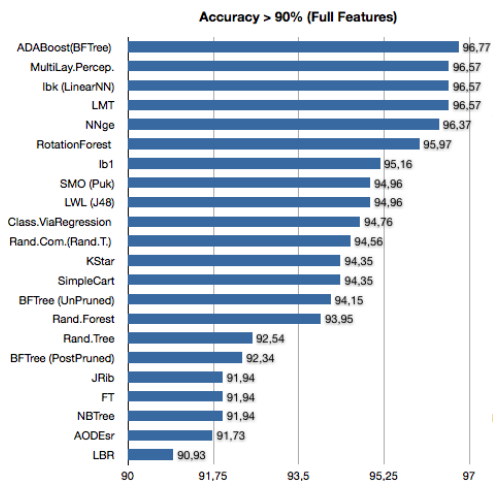
\includegraphics[width=1\textwidth]{accuracy_a.png}
    \caption{Sa svim atributima}

\end{subfigure}
~
\begin{subfigure}[t]{\figWidth}
    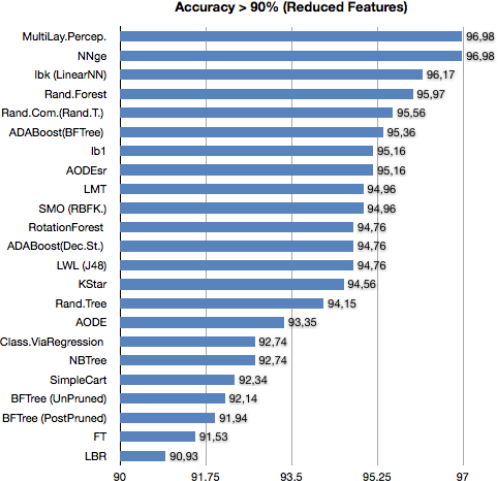
\includegraphics[width=1\textwidth]{accuracy_b.png}
    \caption{Sa redukovanim skupom atributa}

\end{subfigure}

\caption{Preciznost klasifikacije u zavisnosti od algoritma}

\label{fig:acc}
\end{figure}

% false negative
\begin{figure}[h!]
\centering
\begin{subfigure}[t]{\figWidth}
    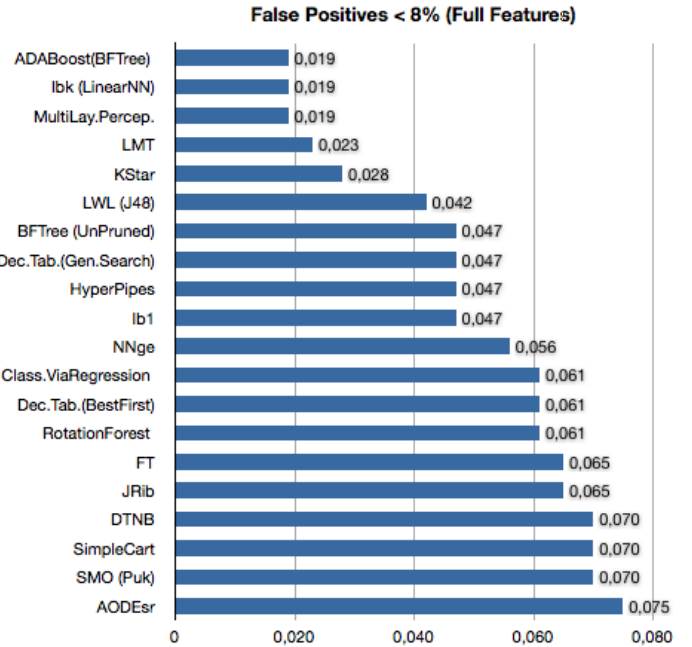
\includegraphics[width=1\textwidth]{false_pos_a.png}
    \caption{Sa svim atributima}

\end{subfigure}
~
\begin{subfigure}[t]{\figWidth}
    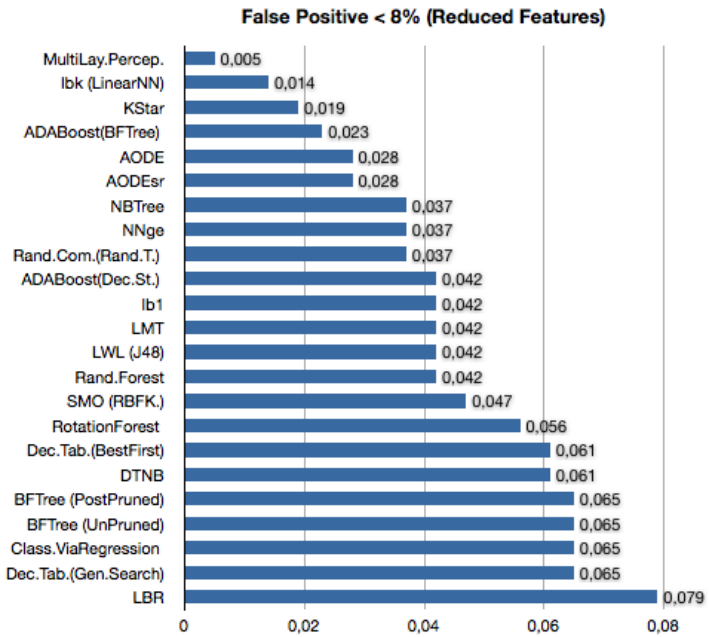
\includegraphics[width=1\textwidth]{false_pos_b.png}
    \caption{Sa redukovanim skupom atributa}

\end{subfigure}

\caption{Udeo lažno pozitivnih instanci u zavisnosti od algoritma}

\label{fig:falsePos}
\end{figure}

% false positive
\begin{figure}[h!]
\centering
\begin{subfigure}[t]{\figWidth}
    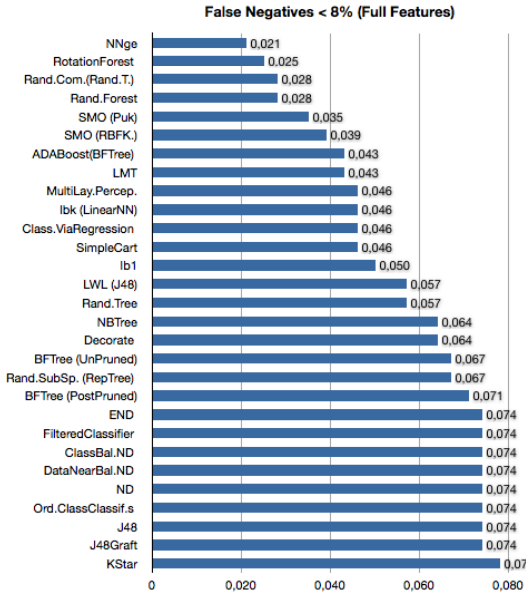
\includegraphics[width=1\textwidth]{false_neg_a.png}
    \caption{Sa svim atributima}

\end{subfigure}
~
\begin{subfigure}[t]{\figWidth}
    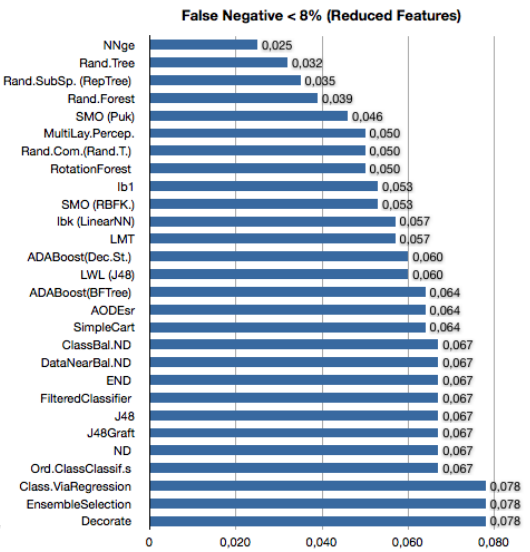
\includegraphics[width=1\textwidth]{false_neg_b.png}
    \caption{Sa redukovanim skupom atributa}

\end{subfigure}

\caption{Udeo lažno negativnih instanci u zavisnosti od algoritma}

\label{fig:falseNeg}
\end{figure}
\end{comment}
\section{Literatura}
\bibliography{seminarski}
\bibliographystyle{plain}

\end{document}